\subsection{Widgets}
\label{subsec:widgets}
Um eine \ac{gui} gestalten zu können braucht es Komponenten, die auf der \ac{gui} angezeigt
werden können. Qt verwendet dafür sogenannte \emph{Widgets}. Widgets sind also grafische
Komponenten, die dafür genutzt werden können, um die Benutzeroberfläche nach belieben zu
gestalten. Ein Beispiel für eine solche Komponente wäre ein Button, welcher in der Sektion
\emph{\nameref{subsec:programmierbeispiel}} als \emph{btnExit} vorkam.
\newline
\newline
Die Widgets, die Qt zur verfügung stellt sind in einer großen Klassenhierarchie zusammengesetzt
und diese Hierarchie könnte sich wie folgt vorgestellt werden:

\begin{figure}[h]
    \centering
    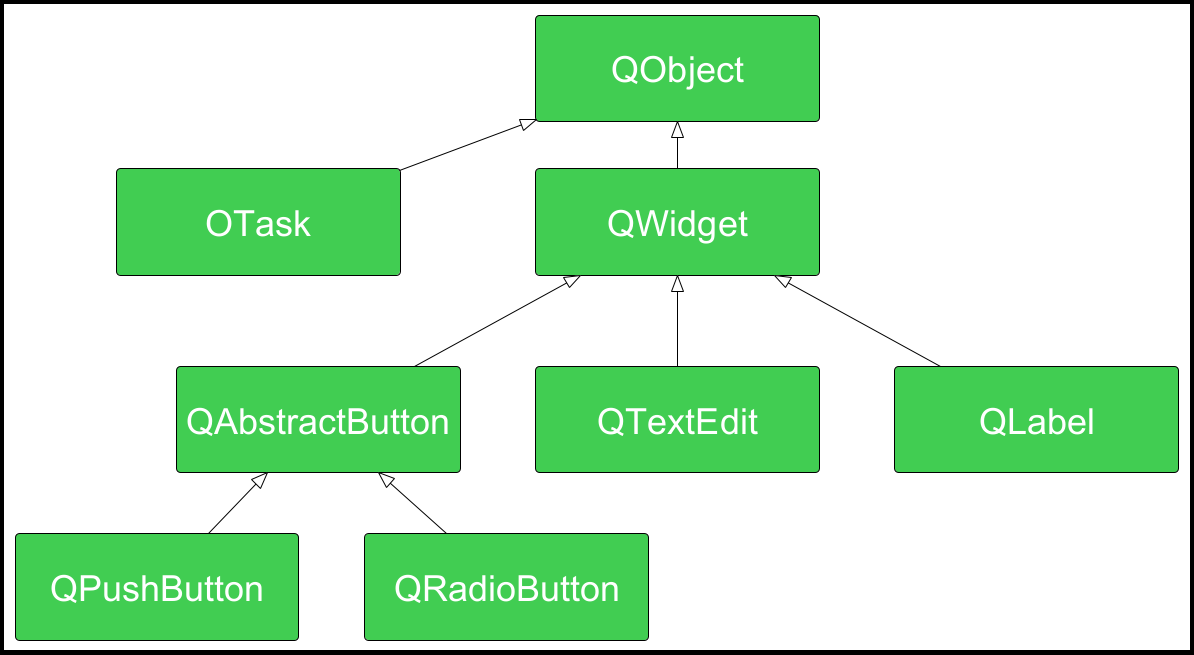
\includegraphics[width=\textwidth, center]{StandDerTechnik/qtWidgetClassHierachie}
    \caption[Qt Widgets Klassenhierachie]{Qt Widgets Klassenhierarchie
    \cite{GettingStartedQt}[vgl.]}
    \label{img:qtWidgetClassHierachie}
\end{figure}

Wie zu sehen ist, ist ganz oben in der Klassenhierarchie die \emph{QObject} Klasse. Diese
enthällt unter anderem den Signal und Slot mechanismus, welcher später noch genau erklärt wird.
Weitergehend, werden Widgets, die gemeinsame Funktionalitäten aufweisen zusammen grupiert. Diese
Verhalten ist bei \emph{QPushButton} und \emph{QRadioButton} erkennbar, denn beide Widgets sind
Buttons, die sich Teilweise die gleichen Eigenschaften und Funktionen teilen
\cite{GettingStartedQt}[vgl.].
